% =============================================================================
%  Radiation Tolerance of the ATLAS TileCal Phase-II Upgrade
%
%  Author:  Róbert Astaloš
%  Style:   tikzposter, A0 portrait, ATLAS colour scheme
% =============================================================================

\documentclass[a0paper,portrait, blockverticalspace=4em, colspace=2em]{tikzposter}
\tikzposterlatexaffectionproofoff
\usepackage{graphicx}
\usepackage{amsmath}
\usepackage{amssymb}
\usepackage{hyperref}
\usepackage{multicol}
\usetikzlibrary{calc}

% ---------------------------------------------------------------------------
%  Colours
% ---------------------------------------------------------------------------
\definecolor{maincolor}{HTML}{9e2b2f}
\definecolor{secondarycolor}{RGB}{158, 43, 47}
\definecolor{lightred}{RGB}{237, 199, 201}

\definecolor{tid}{RGB}{254,128,2}   % orange  — Total Ionizing Dose
\definecolor{niel}{RGB}{0,140,0}    % green   — Non-Ionizing Energy Loss
\definecolor{see}{RGB}{190,0,62}    % red     — Single Event Effects
\definecolor{sel}{RGB}{0,90,170}    % blue    — Single Event Latch-up

% ===========================================================================
%  LAYOUT PARAMETERS
% ===========================================================================
\newcommand{\looseitems}{\small\begin{itemize}\setlength{\itemsep}{0.1em}}
\newcommand{\tightitems}{\small\begin{itemize}\setlength{\itemsep}{0.0em}}
\newcommand{\captiontext}[1]{%
    {\footnotesize\renewcommand{\baselinestretch}{0.88}\selectfont#1}}

% ---------------------------------------------------------------------------
%  Theme
% ---------------------------------------------------------------------------
\usetheme{Default}
\definecolorstyle{atlascolors}{
    \colorlet{backgroundcolor}{white}
    \colorlet{titlefgcolor}{white}
    \colorlet{titlebgcolor}{maincolor}
    \colorlet{blocktitlefgcolor}{white}
    \colorlet{blocktitlebgcolor}{maincolor}
    \colorlet{blockbodyfgcolor}{black}
    \colorlet{blockbodybgcolor}{lightred!25}
}{}
\usecolorstyle{atlascolors}

% Title bar with ATLAS logo
\definetitlestyle{sampletitle}{width=760mm, roundedcorners=20, linewidth=2pt,
  innersep=10pt, titletotopverticalspace=6mm, titletoblockverticalspace=8mm}{%
  \begin{scope}[line width=\titlelinewidth, rounded corners=\titleroundedcorners]
    \draw[color=blocktitlebgcolor, fill=titlebgcolor]
      (\titleposleft,\titleposbottom) rectangle (\titleposright,\titlepostop);
  \end{scope}
  \node[anchor=east, fill=white, rounded corners=10pt, inner sep=10pt, xshift=-22mm]
    at ($(\titleposright,\titlepostop)!0.5!(\titleposright,\titleposbottom)$)
    {
\includegraphics[height=8.6cm]{logos/atlas_transparent.png}};}
\usetitlestyle{sampletitle}

\title{\parbox{0.74\linewidth}{\centering\huge
    System-Level Radiation Tolerance of the\\[2mm]ATLAS TileCal Phase-II Upgrade for the HL-LHC}}
\author{Róbert Astaloš \quad on behalf of the ATLAS Tile Calorimeter System}
\institute{Comenius University Bratislava}
\date{}

\setlength{\columnsep}{0.5cm}

\begin{document}
\maketitle

\begin{columns}

% ===========================================================================
%  COLUMN 1
% ===========================================================================
\column{0.333}

\block{The HL-LHC Challenge}{
    \looseitems
        \item The High-Luminosity Large Hadron Collider (HL-LHC) will deliver an integrated luminosity of $3000\,\text{fb}^{-1}$, presenting an unprecedented radiation challenge for the ATLAS Tile Calorimeter (TileCal).
        \item The on-detector electronics must operate flawlessly for over 10 years without any possibility of maintenance access.
        \item A complete redesign of the readout and power distribution systems was necessitated to handle the severe pile-up and extreme radiation fields.
        \item The upgraded system must digitize analog signals from the photomultiplier tubes (PMTs) at a $40\,\text{MHz}$ sampling rate directly on the detector.
        \item This Phase-II upgrade utilizes a highly modular architecture (Minidrawers) to house the sensitive Front-End (FE) electronics.
    \end{itemize}
    \vspace{0.2cm}
    \begin{center}
    \small
    \resizebox{\linewidth}{!}{
    \begin{tabular}{|p{0.35\linewidth}|p{0.65\linewidth}|}
    \hline
    \textbf{Parameter} & \textbf{HL-LHC Target Value} \\
    \hline
    \textbf{Peak Luminosity} & $7.5 \times 10^{34}\,\text{cm}^{-2}\text{s}^{-1}$ \\
    \hline
    \textbf{Integrated Luminosity} & $3000\,\text{fb}^{-1}$ \\
    \hline
    \textbf{Pile-up ($\mu$)} & $\sim 200$ interactions/crossing \\
    \hline
    \textbf{Operational Lifespan} & 10+ years \\
    \hline
    \textbf{Maintenance Window} & Zero (inaccessible during run) \\
    \hline
    \end{tabular}
    }
    \end{center}
    \vspace{0.1cm}
}

\block{Radiation Architecture and Mitigation}{
    \looseitems
        \item The TileCal electronics are located in the outermost regions of the calorimeter, yet they are exposed to substantial secondary particle cascades.
        \item Extensive Monte Carlo simulations (using FLUKA and Geant4) mapped the radiation field across the entire TileCal volume, identifying critical hot-spots.
        \item The architectural mitigation strategy relies heavily on localized power regulation (Point-of-Load) and completely redundant, radiation-hardened data transmission links.
        \item FPGAs, historically susceptible to \textcolor{see}{Single Event Upsets (SEU)}, were replaced with mitigation-hardened firmwares implementing Triple Modular Redundancy (TMR).
        \item Commercial-Off-The-Shelf (COTS) components were rigorously screened; any lot exhibiting Enhanced Low Dose Rate Sensitivity (ELDRS) was immediately disqualified.
        \item The mechanical layout of the Minidrawers was optimized to provide maximal shielding using the massive structural steel of the TileCal wedges, passively reducing the flux of low-energy hadronic components.
    \end{itemize}
}

\block{System-Level Validation at CHARM}{
    \looseitems
        \item While component-level testing isolated individual vulnerabilities, full system-level validation was performed at the CERN High energy AcceleRator Mixed field (CHARM) facility.
        \item CHARM provides a complex radiation field composed of protons, neutrons, pions, and gammas, accurately mimicking the mixed hadronic/electromagnetic environment of the ATLAS cavern.
        \item Fully assembled prototype Minidrawers, populated with the qualified COTS components, were irradiated while fully powered and actively taking data.
        \item The tests successfully demonstrated that the integrated system architecture, including inter-board communications and high-voltage distribution, remained robust against both cumulative damage and transient Single Event Effects (SEEs).
        \item Long-term tests at CHARM confirmed that the integrated leakage currents of all active components combined do not exceed the thermal dissipation capabilities of the Minidrawer water cooling system.
    \end{itemize}
}

\block{Redundancy and Reliability Strategies}{
    \looseitems
        \item The HL-LHC operating environment presents unprecedented challenges for electronics reliability, particularly given the near-impossibility of physical access for maintenance during standard operational years.
        \item The TileCal Phase-II upgrade architecture employs a multifaceted redundancy strategy to mitigate Single Point of Failures (SPOFs).
        \item The system architecture mandates that critical power lines and data readouts are independently routed. A failure in one Minidrawer segment does not cascade into adjacent modules, preserving the overall calorimetric performance of the detector slice.
        \item Redundant communication links are established between the off-detector backend (TilePPR) and the on-detector front-end (TileCoM). These links utilize inherently radiation-hard optical transceivers, verified up to expected doses with significant safety margins.
        \item Continuous telemetry data allows the Detector Control System (DCS) to monitor the health of all components in real-time. Power consumption, operating voltages, and localized temperatures are tracked, enabling predictive maintenance models to identify degrading components before catastrophic failure.
    \end{itemize}
}

\block{References}{
    \small
    \begin{enumerate}\setlength{\itemsep}{0.1em}
        \item E. Valdes (ATLAS), \emph{Irradiation studies and design optimization
        of the ATLAS Tile Calorimeter for the HL-LHC}, IEEE NSS MIC RTSD 2025.
        \item ATLAS Collaboration, \emph{Technical Design Report for the Phase-II
        Upgrade of the ATLAS Tile Calorimeter}, CERN-LHCC-2017-019 (2018).
    \end{enumerate}
}

% ===========================================================================
%  COLUMN 2
% ===========================================================================
\column{0.333}

\block{Minidrawer Electronics Architecture}{
    \tightitems
        \item The Phase-II readout is divided into four autonomous Minidrawers per module, servicing up to 12 PMTs each.
        \item Each Minidrawer incorporates a Main Board housing two Kintex Ultrascale FPGAs, handling local data aggregation, pipeline buffering, and gigabit optical transmission to the off-detector processors.
        \item The Daughterboard (DB) acts as the critical nexus for signal conditioning and digitization.
        \item Continuous operation requires the complete elimination of Single Point of Failures (SPOFs); thus, data links are fully redundant.
    \end{itemize}
    \vspace{0.1cm}
    \begin{center}
        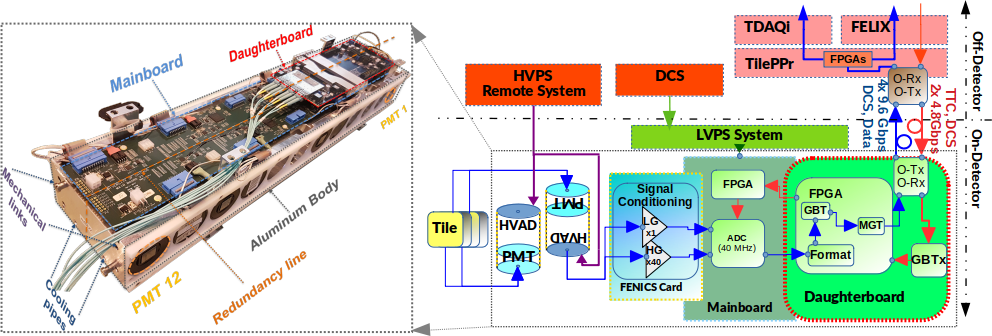
\includegraphics[width=1.0\linewidth]{assets/fig_minidrawer_blockdiagram.png}
    \end{center}
    \vspace{-0.3cm}
    \captiontext{Simplified block diagram of the Minidrawer electronic architecture.}
}

\block{Daughterboard Redesign (DB6)}{
    \tightitems
        \item The Daughterboard (DB) underwent significant iterative optimization, culminating in the final DB6 production version.
        \item DB6 addresses previously identified radiation vulnerabilities, particularly focusing on the Point-of-Load (PoL) regulators.
        \item The integration of radiation-hardened components, specifically the bPOL12V and bPOL2V5 regulators, significantly enhanced immunity against \textcolor{tid}{TID} and \textcolor{sel}{SEL}.
        \item The DB6 design guarantees uninterrupted $40\,\text{MHz}$ digitization and transmission even under peak expected pile-up scenarios.
    \end{itemize}
    \vspace{0.1cm}
    \begin{center}
        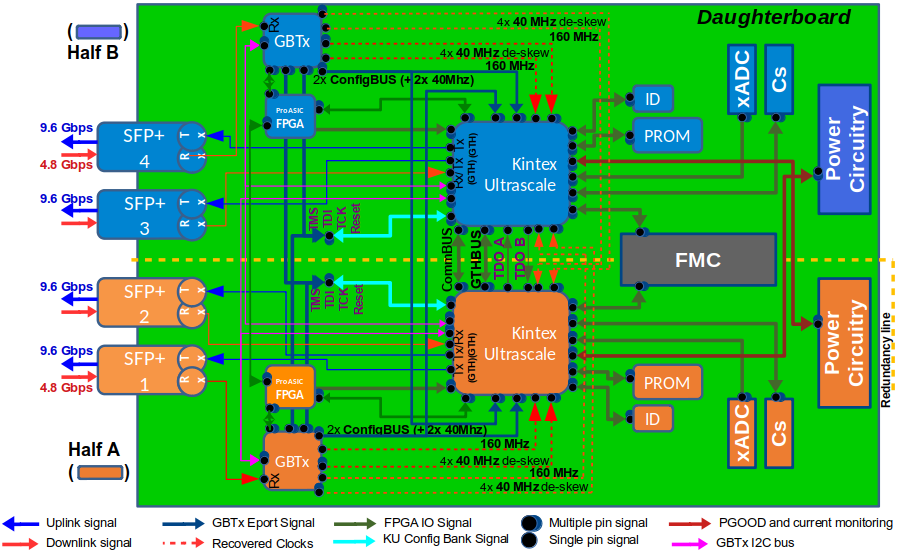
\includegraphics[width=1.0\linewidth]{assets/fig_db6_blockdiagram.png}
    \end{center}
    \vspace{-0.3cm}
    \captiontext{Detailed schematic architecture of the final Daughterboard 6 (DB6) iteration.}
}

\block{Thermal and Electrical Stress Testing}{
    \tightitems
        \item Beyond radiation, the DB6 and Minidrawer assemblies were subjected to extreme thermal and electrical stress tests to simulate worst-case scenarios inside the detector.
        \item Power cycling tests over hundreds of iterations verified the structural integrity of the high-density BGA soldering, preventing fatigue failures.
        \item Over-voltage injection and rapid transient response analyses confirmed that the internal protection circuits trip effectively, isolating faults before they can damage upstream detector infrastructure.
        \item Accelerated aging tests in climatic chambers demonstrated that the FR4 PCB substrate and conformal coatings do not degrade mechanically or electrically over the equivalent of 15 years of operational stress.
    \end{itemize}
    \vspace{0.2cm}
    \begin{center}
    \small
    \resizebox{\linewidth}{!}{
    \begin{tabular}{|p{0.35\linewidth}|p{0.65\linewidth}|}
    \hline
    \textbf{Test Category} & \textbf{Validation Metric} \\
    \hline
    \textbf{Thermal Cycling} & $0^\circ\text{C}$ to $60^\circ\text{C}$, 500 cycles \\
    \hline
    \textbf{Power Integrity} & $<1\%$ ripple at full load \\
    \hline
    \textbf{Over-voltage} & $150\%$ nominal voltage survival \\
    \hline
    \textbf{Signal Integrity} & Bit Error Rate $<10^{-12}$ \\
    \hline
    \textbf{Vibration Analysis} & Passed $3g$ random vibration \\
    \hline
    \textbf{EMC Compliance} & Conducted/radiated emissions pass \\
    \hline
    \textbf{Burn-in Phase} & 72 hours continuous operation \\
    \hline
    \end{tabular}
    }
    \end{center}
    \vspace{0.1cm}
}

\block{FPGA Firmware Migration and TMR Strategy}{
    \tightitems
        \item The Phase-II readout system heavily relies on Kintex Ultrascale FPGAs for massive parallel data processing.
        \item Standard commercial FPGAs are highly vulnerable to \textcolor{see}{SEE}, requiring complex mitigation techniques directly coded into the hardware description language.
        \item Triple Modular Redundancy (TMR) was universally applied to all critical state machines and configuration registers, ensuring that single bit flips are outvoted by redundant parallel logic blocks.
        \item The bitstream scrubbing mechanism continuously monitors and repairs the configuration memory in the background, without interrupting the active data acquisition pipeline.
        \item Validation of the TMR firmware was explicitly performed under heavy ion and proton beams, confirming an error cross-section that aligns with the 10-year MTBF target.
    \end{itemize}
}

% ===========================================================================
%  COLUMN 3
% ===========================================================================
\column{0.333}

\block{Daughterboard Irradiation Performance}{
    \looseitems
        \item The final DB6 prototype was rigorously validated under high-flux \textcolor{tid}{TID} conditions to verify its long-term operational stability.
        \item Testing confirmed that the optical transceivers and FPGAs maintain deterministic latency and zero data-corruption rates up to extreme dose levels.
        \item Analog-to-Digital Converter (ADC) baseline shifts were minimal and easily correctable via offline calibration routines, preserving the required $1\%$ energy resolution.
    \end{itemize}
    \vspace{0.1cm}
    \begin{center}
        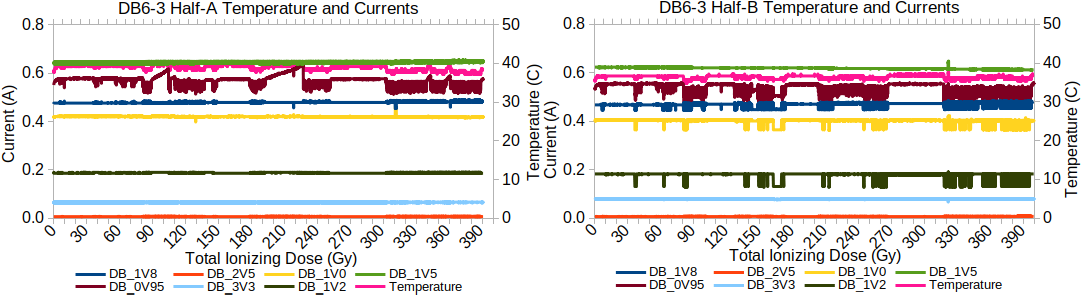
\includegraphics[width=1.0\linewidth]{assets/fig_db6_tid_test.png}
    \end{center}
    \vspace{-0.3cm}
    \captiontext{DB6 system performance stability under accumulated \textcolor{tid}{TID}.}
}

\block{Dose Margins and Safety Requirements}{
    \looseitems
        \item To certify components for the HL-LHC, testing must exceed the simulated dose profiles by significant Safety Factors (SF).
        \item For \textcolor{tid}{TID}, the certification threshold is calculated as: $D_{\text{sim}} \times \text{SF}_{\text{sim}} \times \text{SF}_{\text{LDR}}$, accounting for simulation uncertainties and Low Dose Rate effects.
        \item The rigorous component screening enforced a minimum \textcolor{see}{SEE} cross-section constraint, ensuring that the mean time between failures (MTBF) for the entire 256-module calorimeter exceeds the 10-year operational lifespan.
        \item Final integrated validation tests demonstrated that the system operates with substantial margin beyond the $80\,\text{Gy}$ \textcolor{tid}{TID} specification baseline without requiring any active intervention or recalibration.
    \end{itemize}
}

\block{Global Manufacturing and QA Strategy}{
    \looseitems
        \item The transition from prototype validation to mass production requires a distributed Quality Assurance (QA) pipeline.
        \item Components are batch-tested upon reception. Fully assembled DB6 boards are subjected to automated functional tests utilizing standardized test-benches before integration into the Minidrawers.
        \item Minidrawers undergo a final 72-hour thermal burn-in cycle before shipment to CERN for insertion into the TileCal super-drawers.
        \item This comprehensive QA methodology minimizes infant mortality rates and guarantees the reliability of the installed system.
    \end{itemize}
    \vspace{0.2cm}
    \begin{center}
    \small
    \resizebox{\linewidth}{!}{
    \begin{tabular}{|p{0.35\linewidth}|p{0.65\linewidth}|}
    \hline
    \textbf{QA Stage} & \textbf{Rejection Threshold} \\
    \hline
    \textbf{Component Screening} & Any deviation $>5\%$ from spec \\
    \hline
    \textbf{Bare Board Testing} & $>0.1\,\Omega$ trace resistance \\
    \hline
    \textbf{Functional Testing} & Any failed diagnostic register \\
    \hline
    \textbf{Burn-in Phase} & Failure during 72h thermal load \\
    \hline
    \textbf{Final Integration} & Connector insertion failure \\
    \hline
    \textbf{Shipping Prep} & ESD packaging breach \\
    \hline
    \textbf{Cavern Reception} & Failed visual/electrical test \\
    \hline
    \textbf{Long-term QA} & Drift in telemetry parameters \\
    \hline
    \textbf{Module Assembly} & Physical clearance violation \\
    \hline
    \end{tabular}
    }
    \end{center}
    \vspace{0.1cm}
}

\block{Conclusions}{
    \looseitems
        \item The ATLAS TileCal Phase-II electronics have successfully passed all system-level radiation qualification milestones.
        \item The DB6 architectural iteration resolved all previously identified single-point vulnerabilities.
        \item The demonstrated radiation tolerance heavily exceeds the stringent HL-LHC requirements, green-lighting the commencement of full-scale mass production.
        \item Final production modules are currently undergoing their global assembly phase, ready for the upcoming Long Shutdown period.
    \end{itemize}
}

\block{Final Detector Assembly and Deployment}{
    \looseitems
        \item The validated TileCal Minidrawers are currently in the final phases of mass assembly at staging facilities worldwide.
        \item Integration into the super-drawers involves precise mechanical alignment and the connection of hundreds of optical fibers per module.
        \item The robust architecture ensures that the full detector array will be ready for the critical path installation during the Long Shutdown 3 (LS3) period.
    \end{itemize}
    \vspace{0.2cm}
    \begin{center}
    \small
    \resizebox{\linewidth}{!}{
    \begin{tabular}{|p{0.35\linewidth}|p{0.65\linewidth}|}
    \hline
    \textbf{Deployment Stage} & \textbf{Status and Metric} \\
    \hline
    \textbf{Design Validation} & 100\% Complete (CHARM) \\
    \hline
    \textbf{Component Screening} & 100\% Complete (Batch Tested) \\
    \hline
    \textbf{DB6 Mass Production} & In Progress ($>50\%$ yielded) \\
    \hline
    \textbf{Minidrawer Assembly} & Commencing globally \\
    \hline
    \textbf{Super-drawer Integration} & Scheduled for CERN staging \\
    \hline
    \textbf{HL-LHC First Beam} & Target operational readiness \\
    \hline
    \end{tabular}
    }
    \end{center}
    \vspace{0.1cm}
}

\end{columns}
\end{document}
